\section{Implementation}

\subsection{Implementation of Design 1}
The PyBullet environment for testing this design consists of a table, soft ball and a robotiq 140 gripper Fig \ref{fig:pybullet_env_design_one}. The table and gripper were imported using a Unified Robot Description Format (URDF) an XML-based file format used to describe the physical and kinematic properties of a robot. The soft ball was created using open source 3D moddeling software - Blender. Multiple balls were created using icosphere mesh with varying subdivision setting. Increasing subdivisions increases the resolution of the mesh, making the ball appear smoother, but it also increases the vertex count potentially making soft body simulation unstable or slower. The blender file exported as .obj provides only the surface mech. To obtain volumetric mesh needed to simulate the soft body, open source software - GMSH was used. 

\begin{figure}[!h!t]
  \centering
  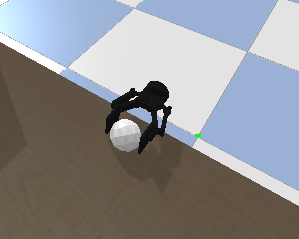
\includegraphics[width=0.4\linewidth]{chapters/exoskeleton/images/background/pybullet_design_one_minimal_setup.png}
  \caption{PyBullet environment for testing \nameone}
  \label{fig:pybullet_env_design_one}
\end{figure}

\bigskip \noindent
The gripper has stroke range of 0 to 0.127 units in the simulation. It is controlled by a single motor using position control. A function that controls the robotiq gripper based on distance instead of angle was created by linearly spacing 100 points of gripper's stroke range, measuring the angle of the motor and the distance between the fingerpads in simulation and fitting this data using a polynomial Fig \ref{fig:robotiq_polynomial_fit}.

\begin{figure}[!h!t]
  \centering
  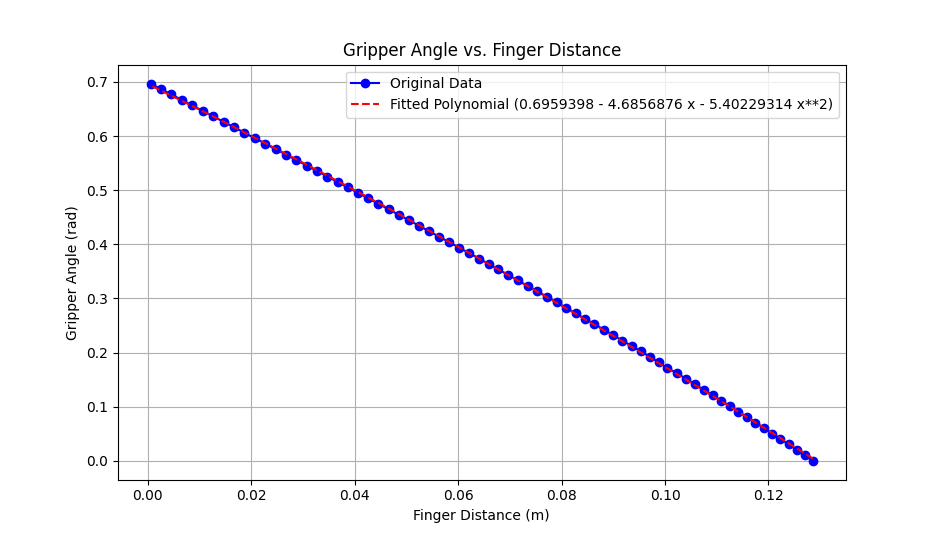
\includegraphics[width=0.8\linewidth]{chapters/exoskeleton/images/background/polynomial_fitting_robotiq.png}
  \caption{Polynomial fitting between gripper's angle and distance}
  \label{fig:robotiq_polynomial_fit}
\end{figure}

\bigskip \noindent
The Dynamixel motors are controlled with the python files provided in their SDK.
The distance between finger pads can be calculated using simple trigonometry Eq \ref{eq:trigonometry_distance_prototype1}, Fig \ref{fig:trigonometry_distance_prototype1}. This distance obtained from the motors is scaled and applied to the simulation every frame.

\begin{equation}
  \label{eq:trigonometry_distance_prototype1}
  \begin{aligned}
      p_1 &= r_1 \cdot \cos(a_1) \\
      p_2 &= r_2 \cdot \cos(a_2) \\
      d_{total} &= -p_1 + d_0 + p_2 
  \end{aligned}
  \end{equation}

\begin{figure}[!h!t]
  \centering
  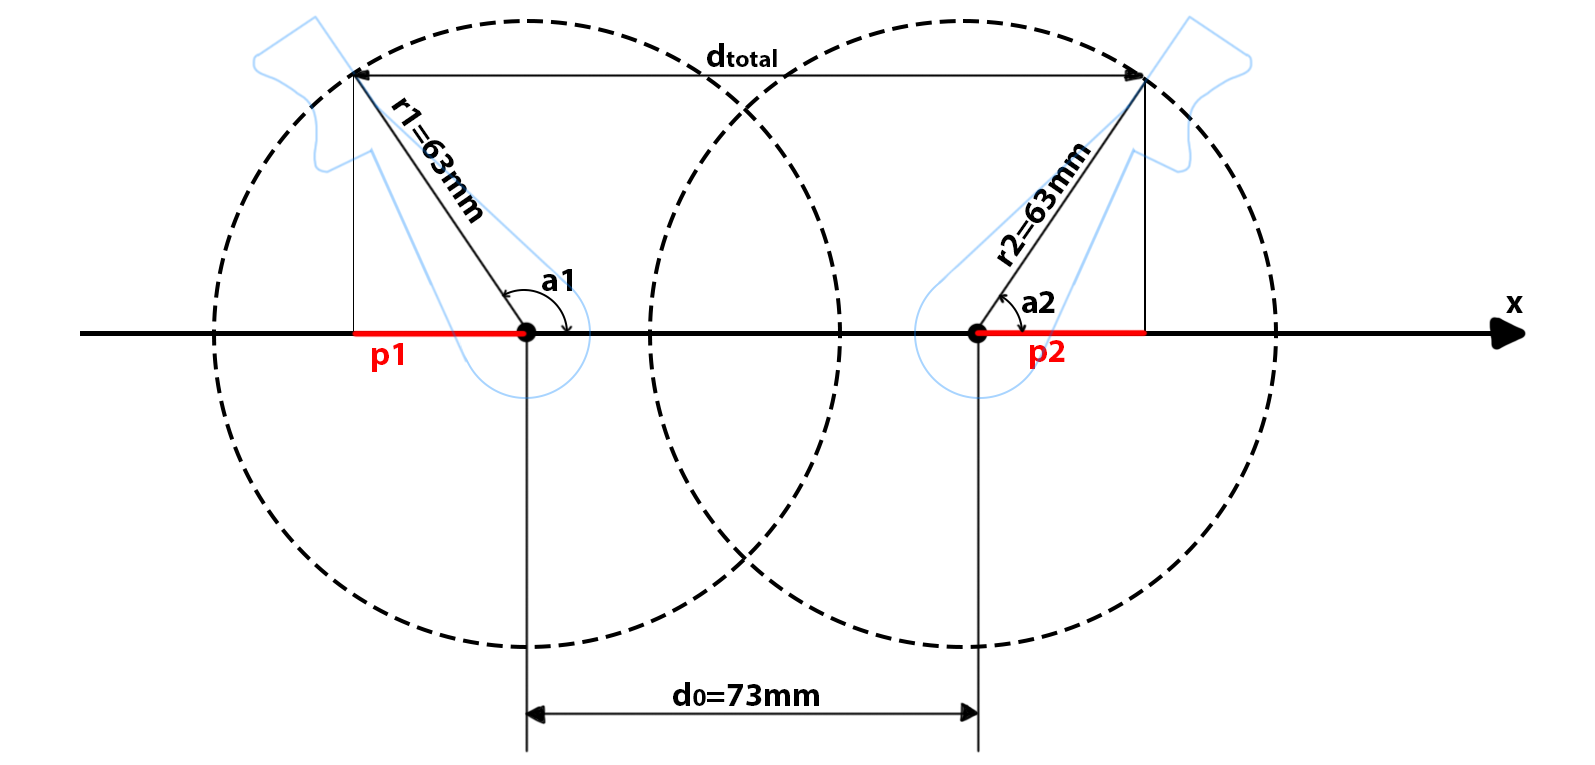
\includegraphics[width=0.8\linewidth]{chapters/exoskeleton/images/background/prototype1_trigonometry.png}
  \caption{Diagram of distance calculation for \nameone}
  \label{fig:trigonometry_distance_prototype1}
\end{figure}

\bigskip \noindent
about getting soft body simulation and vr to work...

\bigskip \noindent
about using force measurement and converting it to torque

\bigskip \noindent
about controllers